% Options for packages loaded elsewhere
\PassOptionsToPackage{unicode}{hyperref}
\PassOptionsToPackage{hyphens}{url}
%
\documentclass[
  ignorenonframetext,
  aspectratio=169,
]{beamer}
\usepackage{pgfpages}
\setbeamertemplate{caption}[numbered]
\setbeamertemplate{caption label separator}{: }
\setbeamercolor{caption name}{fg=normal text.fg}
\beamertemplatenavigationsymbolsempty
% Prevent slide breaks in the middle of a paragraph
\widowpenalties 1 10000
\raggedbottom
\setbeamertemplate{part page}{
  \centering
  \begin{beamercolorbox}[sep=16pt,center]{part title}
    \usebeamerfont{part title}\insertpart\par
  \end{beamercolorbox}
}
\setbeamertemplate{section page}{
  \centering
  \begin{beamercolorbox}[sep=12pt,center]{section title}
    \usebeamerfont{section title}\insertsection\par
  \end{beamercolorbox}
}
\setbeamertemplate{subsection page}{
  \centering
  \begin{beamercolorbox}[sep=8pt,center]{subsection title}
    \usebeamerfont{subsection title}\insertsubsection\par
  \end{beamercolorbox}
}
\AtBeginPart{
  \frame{\partpage}
}
\AtBeginSection{
  \ifbibliography
  \else
    \frame{\sectionpage}
  \fi
}
\AtBeginSubsection{
  \frame{\subsectionpage}
}

\usepackage{amsmath,amssymb}
\usepackage{iftex}
\ifPDFTeX
  \usepackage[T1]{fontenc}
  \usepackage[utf8]{inputenc}
  \usepackage{textcomp} % provide euro and other symbols
\else % if luatex or xetex
  \usepackage{unicode-math}
  \defaultfontfeatures{Scale=MatchLowercase}
  \defaultfontfeatures[\rmfamily]{Ligatures=TeX,Scale=1}
\fi
\usepackage{lmodern}
\usetheme[]{Frankfurt}
\usefonttheme{structurebold}
\ifPDFTeX\else  
    % xetex/luatex font selection
\fi
% Use upquote if available, for straight quotes in verbatim environments
\IfFileExists{upquote.sty}{\usepackage{upquote}}{}
\IfFileExists{microtype.sty}{% use microtype if available
  \usepackage[]{microtype}
  \UseMicrotypeSet[protrusion]{basicmath} % disable protrusion for tt fonts
}{}
\makeatletter
\@ifundefined{KOMAClassName}{% if non-KOMA class
  \IfFileExists{parskip.sty}{%
    \usepackage{parskip}
  }{% else
    \setlength{\parindent}{0pt}
    \setlength{\parskip}{6pt plus 2pt minus 1pt}}
}{% if KOMA class
  \KOMAoptions{parskip=half}}
\makeatother
\usepackage{xcolor}
\newif\ifbibliography
\setlength{\emergencystretch}{3em} % prevent overfull lines
\setcounter{secnumdepth}{-\maxdimen} % remove section numbering


\providecommand{\tightlist}{%
  \setlength{\itemsep}{0pt}\setlength{\parskip}{0pt}}\usepackage{longtable,booktabs,array}
\usepackage{calc} % for calculating minipage widths
\usepackage{caption}
% Make caption package work with longtable
\makeatletter
\def\fnum@table{\tablename~\thetable}
\makeatother
\usepackage{graphicx}
\makeatletter
\newsavebox\pandoc@box
\newcommand*\pandocbounded[1]{% scales image to fit in text height/width
  \sbox\pandoc@box{#1}%
  \Gscale@div\@tempa{\textheight}{\dimexpr\ht\pandoc@box+\dp\pandoc@box\relax}%
  \Gscale@div\@tempb{\linewidth}{\wd\pandoc@box}%
  \ifdim\@tempb\p@<\@tempa\p@\let\@tempa\@tempb\fi% select the smaller of both
  \ifdim\@tempa\p@<\p@\scalebox{\@tempa}{\usebox\pandoc@box}%
  \else\usebox{\pandoc@box}%
  \fi%
}
% Set default figure placement to htbp
\def\fps@figure{htbp}
\makeatother

\makeatletter
\@ifpackageloaded{caption}{}{\usepackage{caption}}
\AtBeginDocument{%
\ifdefined\contentsname
  \renewcommand*\contentsname{Table of contents}
\else
  \newcommand\contentsname{Table of contents}
\fi
\ifdefined\listfigurename
  \renewcommand*\listfigurename{List of Figures}
\else
  \newcommand\listfigurename{List of Figures}
\fi
\ifdefined\listtablename
  \renewcommand*\listtablename{List of Tables}
\else
  \newcommand\listtablename{List of Tables}
\fi
\ifdefined\figurename
  \renewcommand*\figurename{Figure}
\else
  \newcommand\figurename{Figure}
\fi
\ifdefined\tablename
  \renewcommand*\tablename{Table}
\else
  \newcommand\tablename{Table}
\fi
}
\@ifpackageloaded{float}{}{\usepackage{float}}
\floatstyle{ruled}
\@ifundefined{c@chapter}{\newfloat{codelisting}{h}{lop}}{\newfloat{codelisting}{h}{lop}[chapter]}
\floatname{codelisting}{Listing}
\newcommand*\listoflistings{\listof{codelisting}{List of Listings}}
\makeatother
\makeatletter
\makeatother
\makeatletter
\@ifpackageloaded{caption}{}{\usepackage{caption}}
\@ifpackageloaded{subcaption}{}{\usepackage{subcaption}}
\makeatother
\makeatletter
\@ifpackageloaded{fontawesome6}{}{\usepackage{fontawesome6}}
\makeatother

\usepackage{bookmark}

\IfFileExists{xurl.sty}{\usepackage{xurl}}{} % add URL line breaks if available
\urlstyle{same} % disable monospaced font for URLs
\hypersetup{
  pdftitle={Do we feel like we're moving? Explorations on subjective social mobility in Argentina.},
  pdfauthor={José Rodríguez de la Fuente},
  hidelinks,
  pdfcreator={LaTeX via pandoc}}


\title{Do we feel like we're moving? Explorations on subjective social
mobility in Argentina.}
\subtitle{The Future of Social Mobility}
\author{José Rodríguez de la Fuente}
\date{2025-12-03}

\begin{document}
\frame{\titlepage}


\section{Introduction: Why Subjective Social
Mobility?}\label{introduction-why-subjective-social-mobility}

\begin{frame}{Advances in the study of social (occupational) mobility}
\phantomsection\label{advances-in-the-study-of-social-occupational-mobility}
\begin{columns}[T]
\begin{column}{0.5\linewidth}
\textbf{International} (Hout \& DiPrete, 2006):\\
- Social mobility shows a \emph{common pattern}, but its strength varies
across countries and over time.\\
- \emph{Education} is the main factor driving both upward mobility and
the intergenerational reproduction of status.
\end{column}

\begin{column}{0.5\linewidth}
\textbf{Latin America} (Torche, 2015; Solís y Boado, 2016):\\
- \emph{High absolute rates} of intergenerational class mobility,
comparable to those in today's industrialized countries.\\
- \emph{Upward mobility} did not always translate into \emph{higher
incomes}.\\
- Overall \emph{social fluidity} is similar to that of European
countries.\\
- Weak link between \emph{inequality and mobility}.
\end{column}
\end{columns}
\end{frame}

\begin{frame}{Social mobility in the stratification process}
\phantomsection\label{social-mobility-in-the-stratification-process}
\begin{columns}[T]
\begin{column}{0.45\linewidth}
\begin{figure}[H]

{\centering \includegraphics[width=0.7\linewidth,height=\textheight,keepaspectratio]{fuentes/Grusky.png}

}

\caption{Source: based on Grusky (2008)}

\end{figure}%
\end{column}

\begin{column}{0.55\linewidth}
\begin{itemize}
\item
  Mobility studies commonly focus on the relationship between
  \emph{origins and destinations} (2).\\
\item
  It is often assumed that the relationship between \emph{positions and
  outcomes} (1) is constant, even though it actually changes over time.
\item
  Economists simplified this issue by focusing directly on \emph{income
  mobility}.
\end{itemize}
\end{column}
\end{columns}
\end{frame}

\begin{frame}{Why subjective social mobility? (I)}
\phantomsection\label{why-subjective-social-mobility-i}
\begin{columns}[T]
\begin{column}{0.45\linewidth}
\textbf{Diagnosis}:

\begin{itemize}
\item
  There is a gap between how sociology defines class or occupational
  mobility and \emph{how people understand} ``social mobility'' in their
  everyday lives.
\item
  What do people understand as upward or downward mobility? Class?
  Income? Housing? Consumption? Education? Lifestyle?
\end{itemize}
\end{column}

\begin{column}{0.55\linewidth}
\textbf{Subjective social mobility}:

\begin{itemize}
\item
  Allows for addressing the {multidimensionality} of social mobility.

  \begin{itemize}
  \item
    Captures a broader \emph{range of experiences}.
  \item
    Reflects a \emph{cognitive average} of objective mobility
    trajectories.
  \item
    Objective and subjective mobility do not always \emph{align}.
  \end{itemize}
\item
  Possible indicator of \emph{relative deprivation}.
\item
  Is a better \emph{predictor} of attitudes, behaviors, health, and
  well-being.
\end{itemize}
\end{column}
\end{columns}
\end{frame}

\begin{frame}{Why subjective social mobility? (II)}
\phantomsection\label{why-subjective-social-mobility-ii}
\begin{columns}[T]
\begin{column}{0.6\linewidth}
\pandocbounded{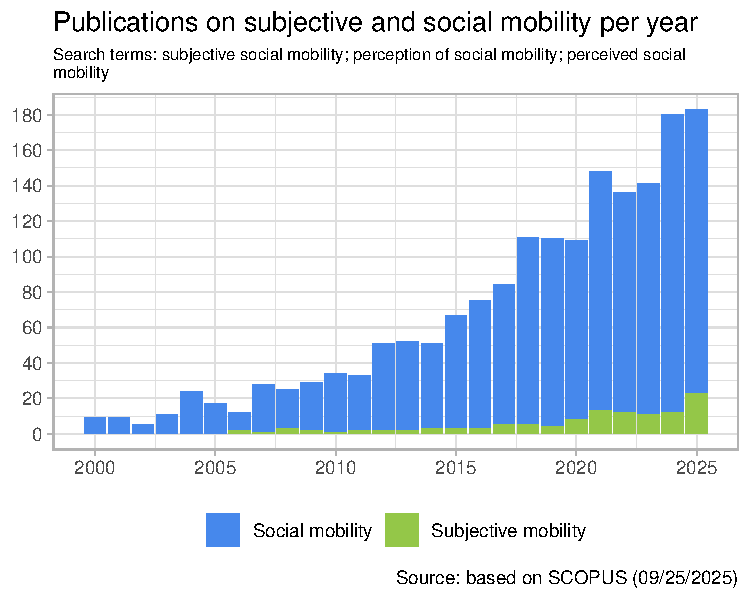
\includegraphics[keepaspectratio]{presentacion_ingles2_files/figure-beamer/Publicaciones por año-1.pdf}}
\end{column}

\begin{column}{0.4\linewidth}
\pandocbounded{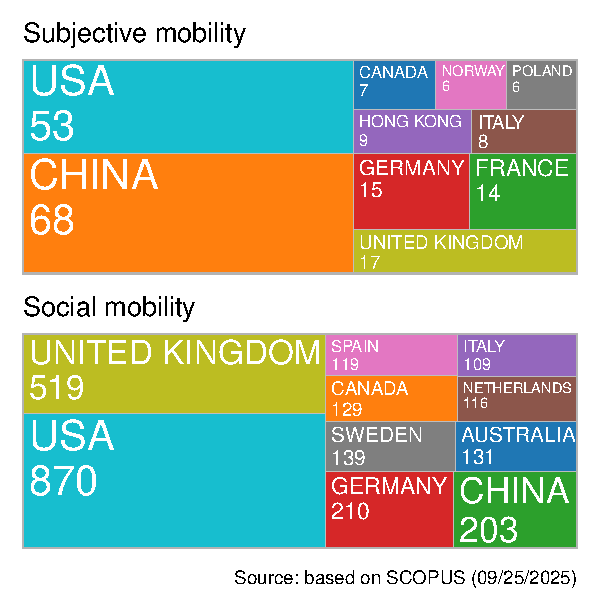
\includegraphics[keepaspectratio]{presentacion_ingles2_files/figure-beamer/Publicaciones por país-1.pdf}}
\end{column}
\end{columns}
\end{frame}

\section{Methodology}\label{methodology}

\begin{frame}{Objectives and data sources}
\phantomsection\label{objectives-and-data-sources}
\begin{columns}[T]
\begin{column}{0.6\linewidth}
\textbf{Objective}: To explore the relationship between objective
indicators of stratification (class and social mobility) and subjective
mobility in Argentina.

\textbf{Data sources}:

\begin{itemize}
\item
  Comparative Analysis: World Values Survey (WVS) and Latinobarómetro.
\item
  Argentina: National Survey on Argentina's Social Structure and
  Equality Policies (ESAyPI, PIRC-ESA, 2024)

  \begin{itemize}
  \tightlist
  \item
    National, urban, probability-based sample
  \item
    1,500 individuals aged 18 and older.
  \end{itemize}
\end{itemize}
\end{column}

\begin{column}{0.4\linewidth}
\begin{itemize}
\tightlist
\item
  \textbf{Direct question} (Qualitative)

  \begin{itemize}
  \tightlist
  \item
    \emph{Comparing your standard of living with your parents' standard
    of living when they were about your age, would you say that you are
    better off, worse off or about the same?}
  \end{itemize}
\end{itemize}

\begin{itemize}
\tightlist
\item
  \textbf{Indirect question} (Quantitative)

  \begin{itemize}
  \tightlist
  \item
    Difference between the subjective status scores of children and
    parents
  \end{itemize}
\end{itemize}
\end{column}
\end{columns}
\end{frame}

\section{Results}\label{results}

\begin{frame}{Subjective mobility in Latin America (I)}
\phantomsection\label{subjective-mobility-in-latin-america-i}
\begin{columns}[T]
\begin{column}{0.5\linewidth}
\pandocbounded{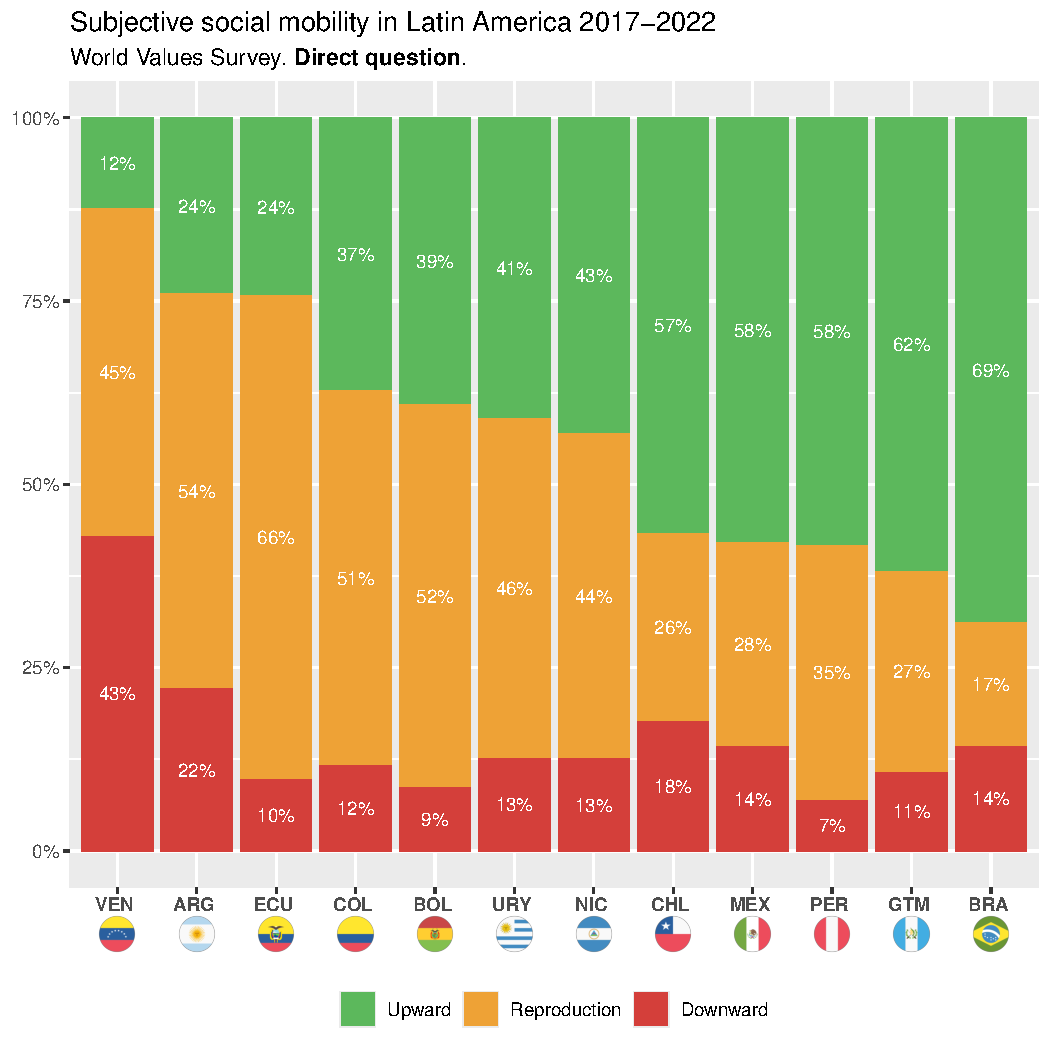
\includegraphics[keepaspectratio]{presentacion_ingles2_files/figure-beamer/Tendencias WVS-1.pdf}}
\end{column}

\begin{column}{0.5\linewidth}
\textbf{World Values Survey}: direct question on subjective mobility

\begin{itemize}
\tightlist
\item
  4 out of 10 people report having improved compared to their parents
\item
  Venezuela, Argentina and Ecuador are the countries with the lowest
  levels of upward subjective mobility
\item
  Brazil, Peru, Mexico and Chile are the countries with the highest
  levels of upward subjective mobility
\end{itemize}
\end{column}
\end{columns}
\end{frame}

\begin{frame}{Subjective mobility in Latin America (II)}
\phantomsection\label{subjective-mobility-in-latin-america-ii}
\begin{columns}[T]
\begin{column}{0.5\linewidth}
\pandocbounded{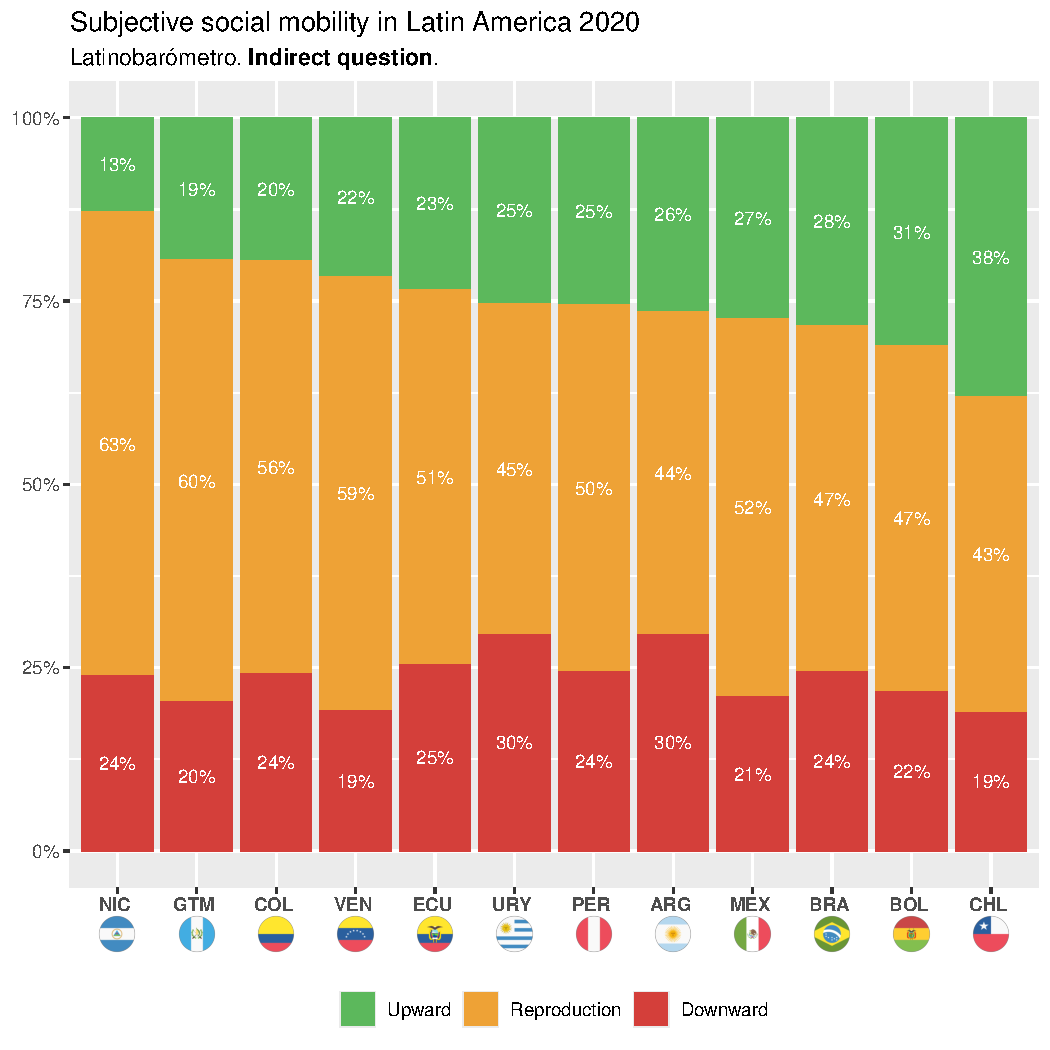
\includegraphics[keepaspectratio]{presentacion_ingles2_files/figure-beamer/Tendencias Latinobarometro-1.pdf}}
\end{column}

\begin{column}{0.5\linewidth}
\textbf{Latinobarómetro}: indirect question on subjective mobility

\begin{itemize}
\tightlist
\item
  1 out of 4 people report having improved compared to their parents
\item
  Social reproduction predominates
\item
  Nicaragua, Colombia and Venezuela are the countries with the lowest
  levels of upward subjective mobility
\item
  Chile, Bolivia and Brazil are the countries with the highest levels of
  upward subjective mobility
\end{itemize}
\end{column}
\end{columns}
\end{frame}

\begin{frame}{Subjective mobility in Argentina (I). Cohorts}
\phantomsection\label{subjective-mobility-in-argentina-i.-cohorts}
\begin{columns}[T]
\begin{column}{0.5\linewidth}
\pandocbounded{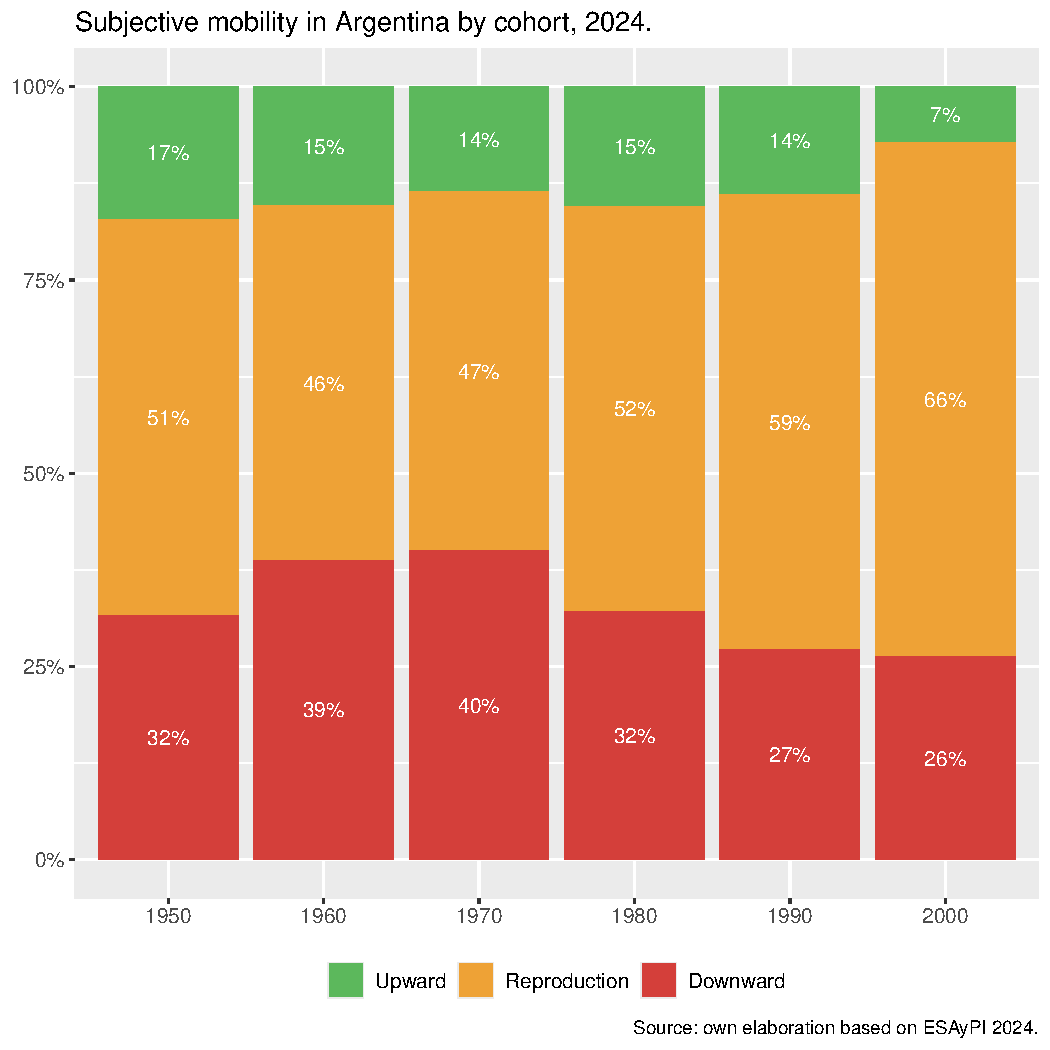
\includegraphics[keepaspectratio]{presentacion_ingles2_files/figure-beamer/Descriptivos Argentina 1-1.pdf}}
\end{column}

\begin{column}{0.5\linewidth}
\begin{itemize}
\tightlist
\item
  The proportion of people who report having experienced \textbf{upward
  mobility} is constant over time (except among the youngest)
\item
  What increases over time is the perception of \textbf{social
  reproduction}
\item
  A mix of generational and life-course effects
\end{itemize}
\end{column}
\end{columns}
\end{frame}

\begin{frame}{Subjective mobility in Argentina (II). Social class}
\phantomsection\label{subjective-mobility-in-argentina-ii.-social-class}
\begin{columns}[T]
\begin{column}{0.5\linewidth}
\pandocbounded{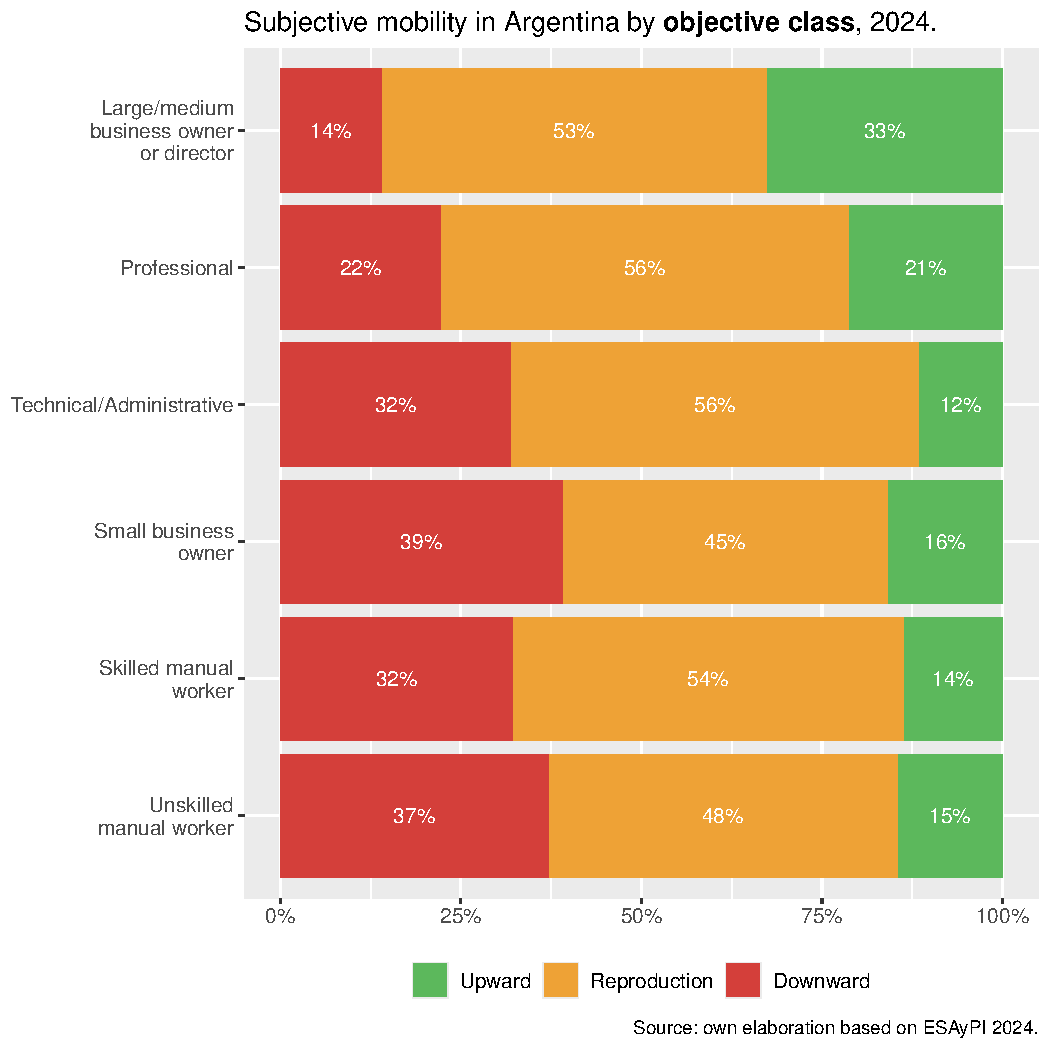
\includegraphics[keepaspectratio]{presentacion_ingles2_files/figure-beamer/Descriptivos Argentina 2.1-1.pdf}}
\end{column}

\begin{column}{0.5\linewidth}
\pandocbounded{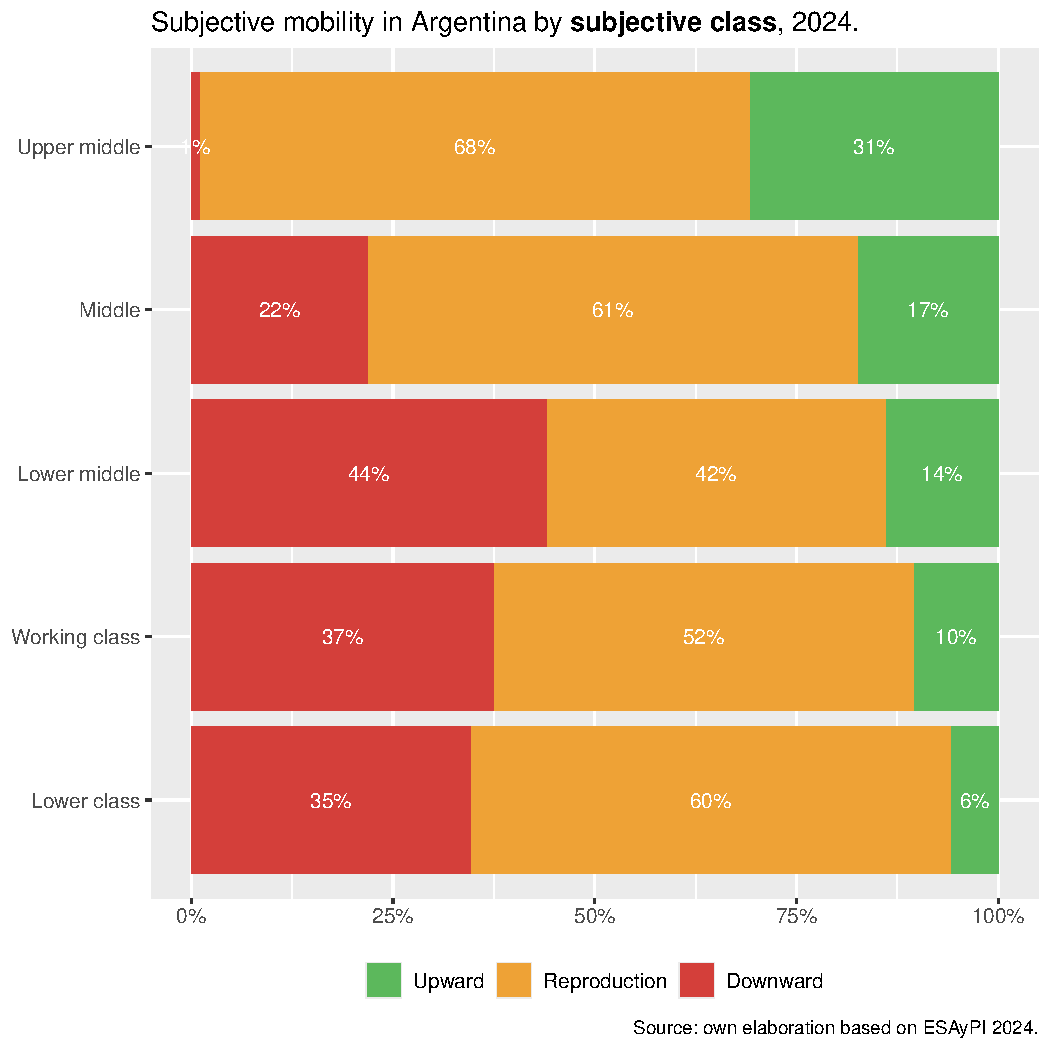
\includegraphics[keepaspectratio]{presentacion_ingles2_files/figure-beamer/Descriptivos Argentina 2.2-1.pdf}}
\end{column}
\end{columns}
\end{frame}

\begin{frame}{Subjective mobility in Argentina (III). Objective social
mobility}
\phantomsection\label{subjective-mobility-in-argentina-iii.-objective-social-mobility}
\begin{columns}[T]
\begin{column}{0.5\linewidth}
\pandocbounded{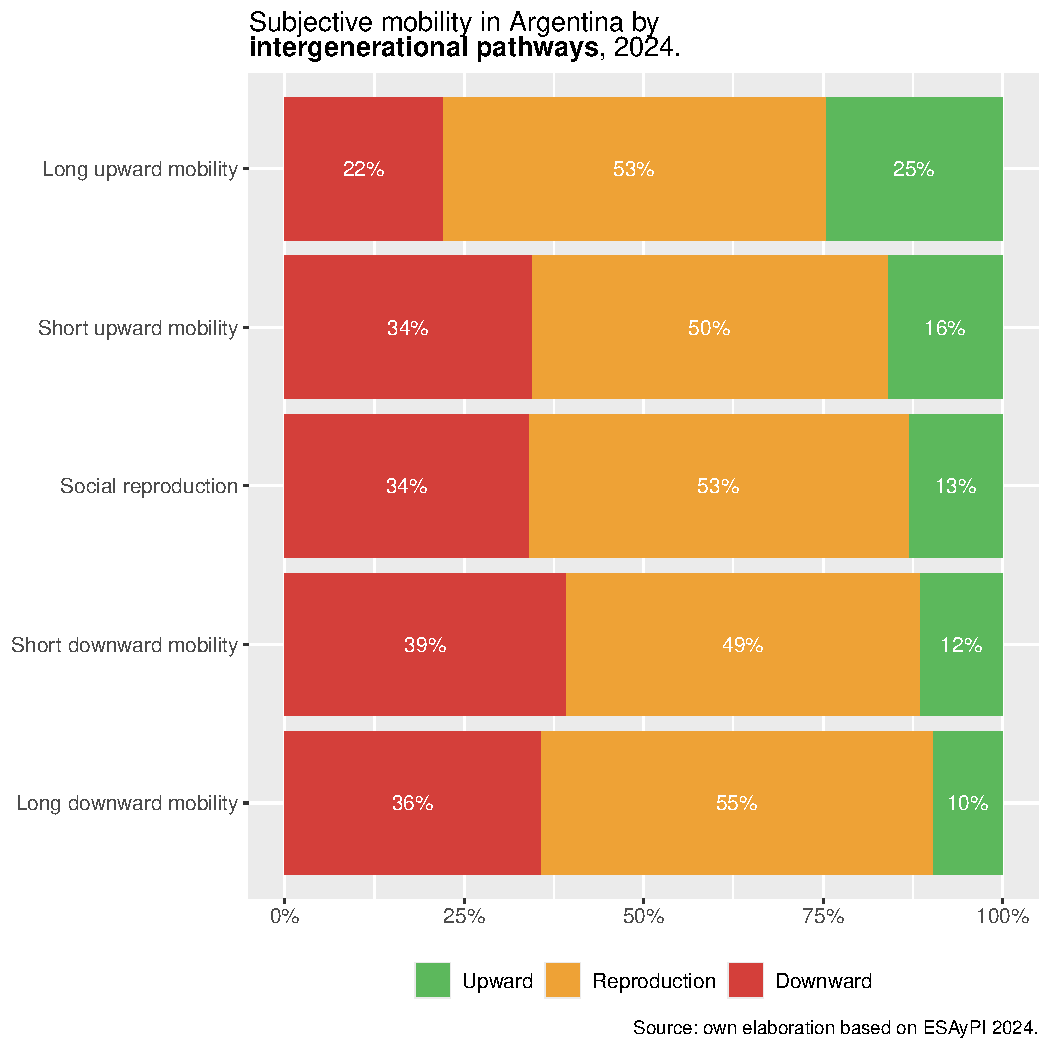
\includegraphics[keepaspectratio]{presentacion_ingles2_files/figure-beamer/Descriptivos Argentina 3-1.pdf}}
\end{column}

\begin{column}{0.5\linewidth}
\begin{itemize}
\tightlist
\item
  There is a partial correspondence between objective and subjective
  mobility.
\item
  When upward objective mobility is more intense, upward subjective
  mobility increases slightly.
\end{itemize}
\end{column}
\end{columns}
\end{frame}

\begin{frame}{Subjective mobility in Argentina (IV). Mobility
explanations}
\phantomsection\label{subjective-mobility-in-argentina-iv.-mobility-explanations}
\begin{columns}[T]
\begin{column}{0.5\linewidth}
\pandocbounded{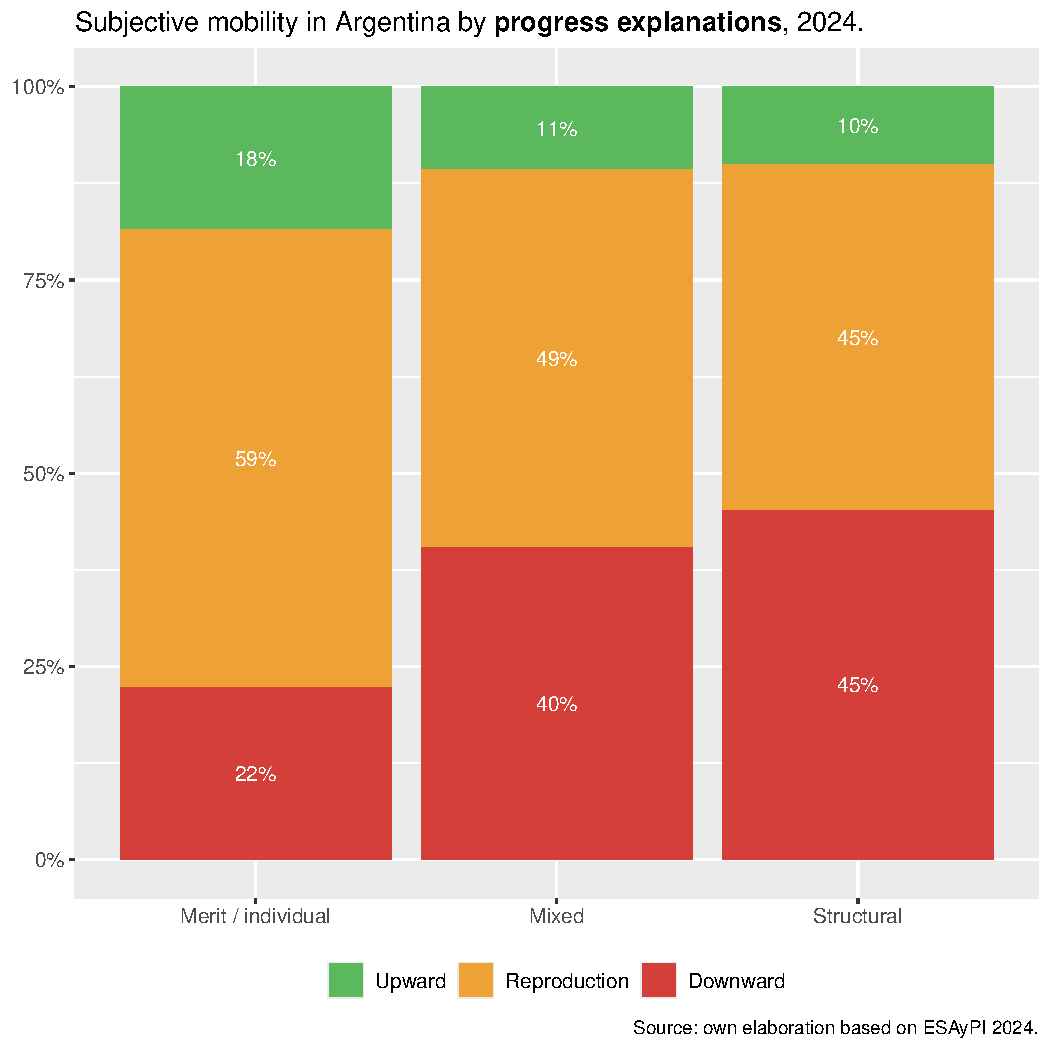
\includegraphics[keepaspectratio]{presentacion_ingles2_files/figure-beamer/unnamed-chunk-1-1.pdf}}
\end{column}

\begin{column}{0.5\linewidth}
\begin{itemize}
\tightlist
\item
  Perceptions of upward mobility and social reproduction are mostly
  linked to individual or \textbf{meritocratic} views of progress, such
  as education, hard work, and ambition.
\item
  Perceptions of downward mobility, in contrast, are more strongly
  associated with \textbf{structural} or \textbf{mixed} explanations of
  the factors shaping progress, such as family background, collective
  organization, or corruption.
\end{itemize}
\end{column}
\end{columns}
\end{frame}

\begin{frame}{Determinants of subjective social mobility}
\phantomsection\label{determinants-of-subjective-social-mobility}
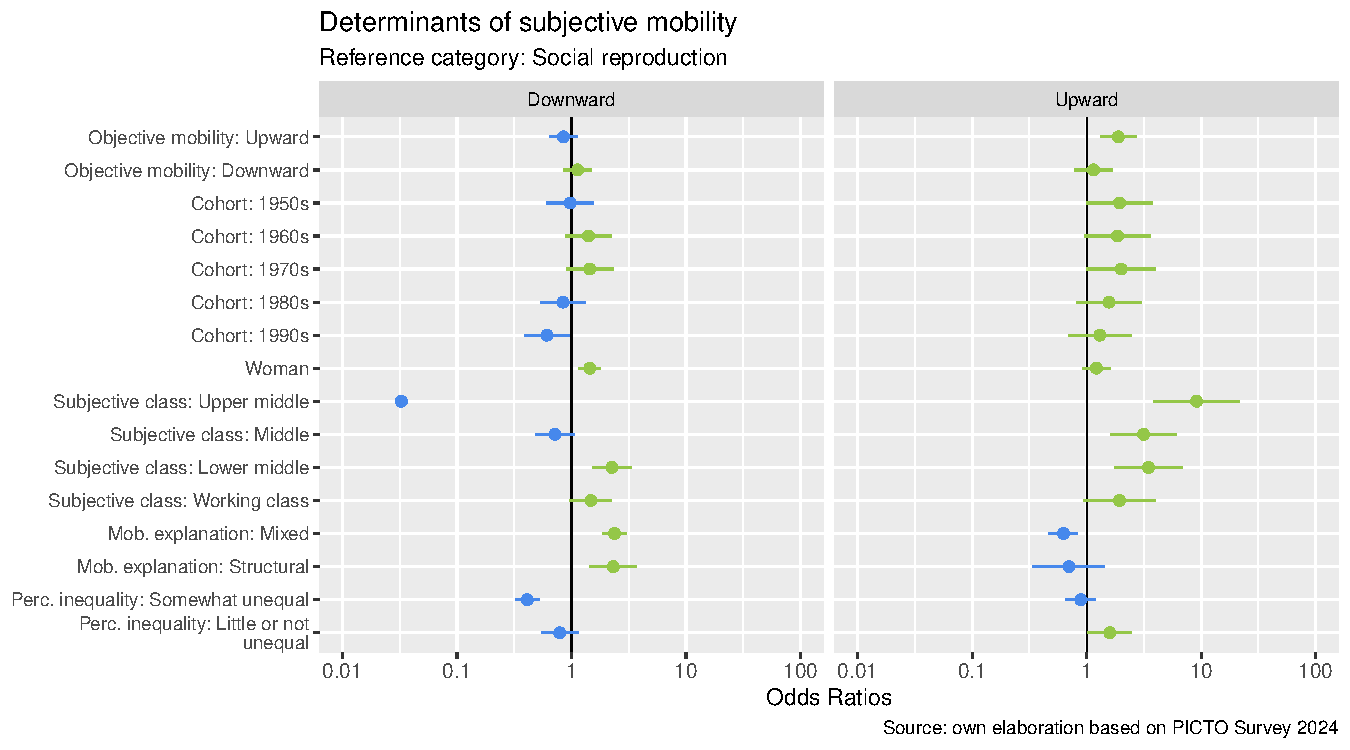
\includegraphics[width=0.95\linewidth,height=\textheight,keepaspectratio]{presentacion_ingles2_files/figure-beamer/Regresión multinomial-1.pdf}
\end{frame}

\section{Conclusions}\label{conclusions}

\begin{frame}{Conclusions and next steps}
\phantomsection\label{conclusions-and-next-steps}
\textbf{Direct vs.~indirect measurement}:

\begin{itemize}
\tightlist
\item
  The direct measure captures more upward mobility, while the indirect
  measure captures more reproduction and downward mobility.
\end{itemize}

\textbf{Argentina}:

\begin{itemize}
\item
  Objective and subjective class positions correlate only weakly with
  subjective mobility.
\item
  Objective mobility does not necessarily translate into subjective
  mobility (\emph{status inconsistency / spurious mobility}).
\item
  Evidence of a \emph{self-serving bias in causal attribution}
  (Structural and merit-based factors).
\end{itemize}

\textbf{Next steps}:

\begin{itemize}
\tightlist
\item
  Further develop subjective mobility measures in household surveys and
  assess how people situate themselves relative to their parents across
  multiple dimensions.
\end{itemize}
\end{frame}

\begin{frame}{}
\phantomsection\label{section}
\begingroup\LARGE Thank you for your attention!\endgroup

\faIcon{envelope} jrodriguez@conicet.gov.ar\\
\faIcon{github-alt} https://github.com/joserodriguez86
\end{frame}




\end{document}
